\documentclass{beamer}
\usepackage[utf8]{inputenc}
\usepackage{amsmath}
\usepackage{mathtools}
\usepackage{bm}
%\usetheme{Berkeley}
\usecolortheme{beaver}

\setbeamercovered{transparent}

\begin{document}

\title{The pinhole camera}
\subtitle{Solving the three geometric problems}
\author{Jarno Leppänen}
\date{13.10.2015}
\frame{\titlepage}

\section{Recap}

\begin{frame}
  \begin{itemize}
  \end{itemize}
\end{frame}

\begin{frame}
  \frametitle{Pinhole Camera Model}
  \begin{align*}
    \mathbf{pinhole}[\mathbf{w},\boldsymbol{\Lambda},\boldsymbol{\Omega},
    \bm{\tau}] &=
      \begin{bmatrix*}[l]
        \frac{\phi_x (\omega_{11}u+\omega_{12}v+\omega_{13}w+\tau_x)
          +\gamma(\omega_{21}u+\omega_{22}v+\omega_{23}w+\tau_y)
        }{\omega_{31}u+\omega_{32}v+\omega_{33}w+\tau_z}+\delta_x \\
        \frac{\phi_y (\omega_{21}u+\omega_{22}v+\omega_{23}w+\tau_y)
        }{\omega_{31}u+\omega_{32}v+\omega_{33}w+\tau_z}+\delta_y \\
      \end{bmatrix} \\
      \\
      \uncover<2->{
    \Pr(\mathbf{x}|\mathbf{w},\boldsymbol{\Lambda},\boldsymbol{\Omega},
    \bm{\tau}) &=
    \operatorname{Norm}_\mathbf{x}[\mathbf{pinhole}[\mathbf{w},
    \boldsymbol{\Lambda},\boldsymbol{\Omega},\bm{\tau}],\sigma^2\mathbf{I}]
  }
  \end{align*}
  \uncover<3->{
  \begin{itemize}
    \item $\boldsymbol{\Lambda}$ are the \emph{intrinsic parameters}
    \item $\boldsymbol{\Omega},\bm{\tau}$ are the \emph{extrinsic parameters}
  \end{itemize}
}
\end{frame}

\begin{frame}
  \frametitle{Learning Extrinsic Parameters}
  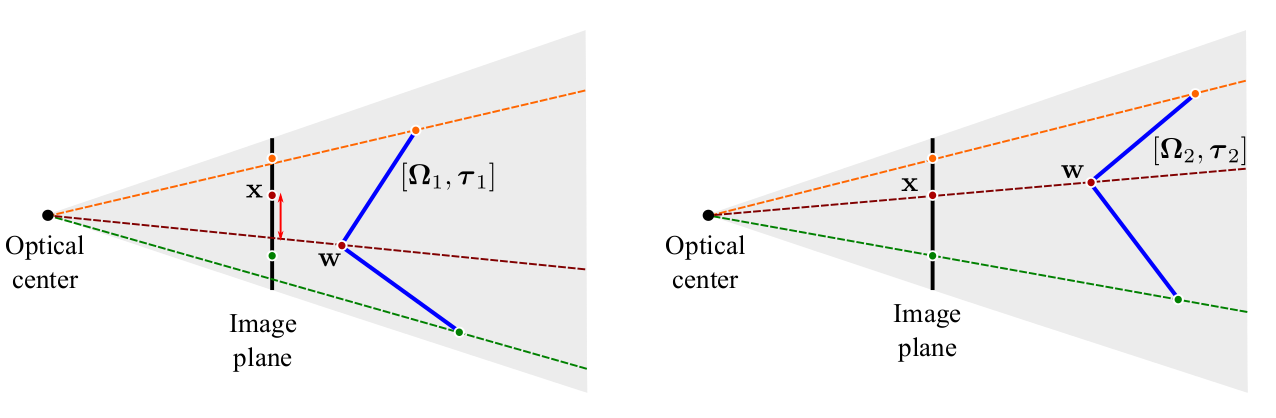
\includegraphics[width=1.0\textwidth]{fig/recap1.png}
  \begin{align*}
    \boldsymbol{\hat{\Omega}},\bm{\hat{\tau}} &=
    \underset{\boldsymbol{\Omega},\bm{\tau}}
    {\operatorname{argmax}} \left[
      \sum_{i=1}^I \log{\left[
    \Pr(\mathbf{x}_i|\mathbf{w}_i,\boldsymbol{\Lambda},\boldsymbol{\Omega},
    \bm{\tau})
      \right]}
    \right]
  \end{align*}
  \begin{itemize}
    \item<2-> $I$ is the number of points
    \item<3-> Position and orientation of the camera
  \end{itemize}
\end{frame}

\begin{frame}
  \frametitle{Learning Intrinsic Parameters}
  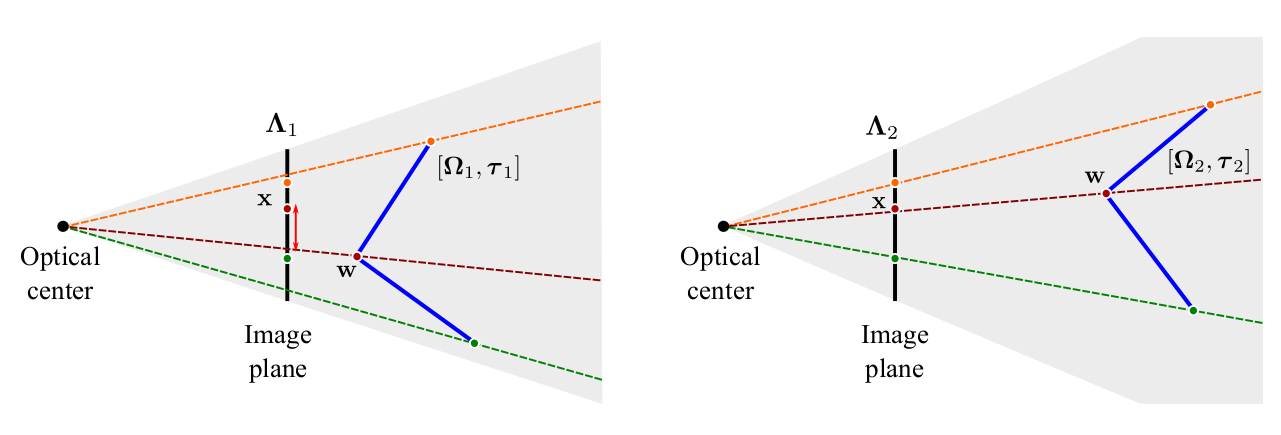
\includegraphics[width=1.0\textwidth]{fig/recap2.png}
  \begin{align*}
    \boldsymbol{\hat{\Lambda}} &=
    \underset{\boldsymbol{\Lambda}}
    {\operatorname{argmax}} \left[
    \underset{\boldsymbol{\Omega},\bm{\tau}}
    {\operatorname{max}} \left[
      \sum_{i=1}^I \log{\left[
    \Pr(\mathbf{x}_i|\mathbf{w}_i,\boldsymbol{\Lambda},\boldsymbol{\Omega},
    \bm{\tau})
      \right]}
  \right]\right]
  \end{align*}
  \begin{itemize}
    \item<2-> $I$ is the number of points
    \item<3-> Focal length and skew calibration
  \end{itemize}
\end{frame}

\begin{frame}
  \frametitle{Inferring 3D World Points}
  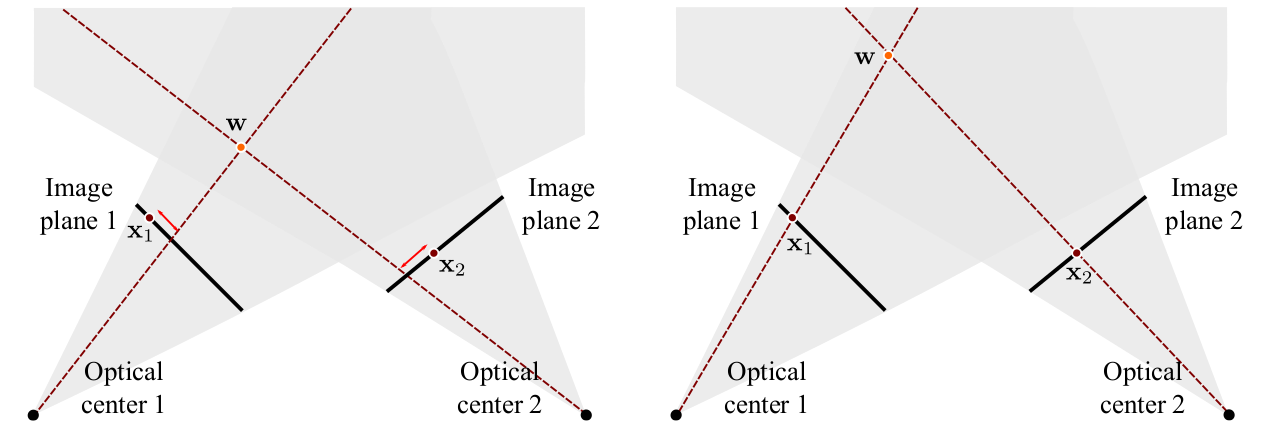
\includegraphics[width=1.0\textwidth]{fig/recap3.png}
  \begin{align*}
    \mathbf{\hat{w}} &=
    \underset{\mathbf{w}}
    {\operatorname{argmax}} \left[
      \sum_{j=1}^J \log{\left[
    \Pr(\mathbf{x}_j|\mathbf{w},\boldsymbol{\Lambda}_j,\boldsymbol{\Omega}_j,
    \bm{\tau}_j)
      \right]}
  \right]
  \end{align*}
  \begin{itemize}
    \item<2-> $J \geq 2$ is the number of cameras
    \item<3-> 3D object reconstruction
  \end{itemize}
\end{frame}

\begin{frame}
  \frametitle{Solving the Problems}
  \begin{itemize}[<+->]
    \item Each objective function is nonconvex
    \item No closed form optimal solutions
    \item Need nonlinear optimization
    \item Need good initial estimates to ensure convergence to global maximum
  \end{itemize}
\end{frame}

\begin{frame}
  \frametitle{Strategy}
  \begin{itemize}[<+->]
    \item Choose new easier objective functions with closed form solutions
    \item Use output as an initial guess to the nonlinear optimization procedure
    \item Find global optimum to the true objective function
  \end{itemize}
\end{frame}

\section{Homogeneous Coordinates}

\begin{frame}
  \frametitle{Homogeneous Coordinates}
  \begin{itemize}[<+->]
    \item Change the representation of 2D and 3D points
    \item Projection equations become linear with the new representation
    \item Resulting modified objective functions minimize a different
      error measure
    \item Solutions are \emph{not} guaranteed to be the same as those for the
      original problem
  \end{itemize}
\end{frame}

\begin{frame}
  \frametitle{Definition}
  \begin{itemize}[<+->]
    \item 2D homogeneous coordinate: $
    \mathbf{\tilde{x}} =
    \begin{bmatrix}
      \tilde{x} \\ \tilde{y} \\ \tilde{z}
    \end{bmatrix}
      = \lambda
    \begin{bmatrix}
      x \\ y \\ 1
    \end{bmatrix}$
  \item Redundant, e.g. $\mathbf{\tilde{x}} = [2,4,2]^T$ and
  $\mathbf{\tilde{x}} = [3,6,3]^T$ both represent the 2D image point
  $\mathbf{x} = [1,2]^T$
\item Conversion to 2D image point: $\mathbf{x} = \begin{bmatrix}
    \tilde{x}/\tilde{z} \\ \tilde{y}/\tilde{z}
  \end{bmatrix}
  $
\item 3D points analogously: $
    \mathbf{\tilde{w}} =
      \lambda
    \begin{bmatrix}
      u \\ v \\ w \\ 1
    \end{bmatrix}$
\end{itemize}
\end{frame}

\begin{frame}
  \frametitle{Geometric Interpretation}
  \begin{columns}
    \column{.5\textwidth}
    \begin{itemize}[<+->]
      \item Homogeneous coordinate defines a ray through the origin
      \item Can represent points at infinity
    \end{itemize}
    \column{.5\textwidth}
      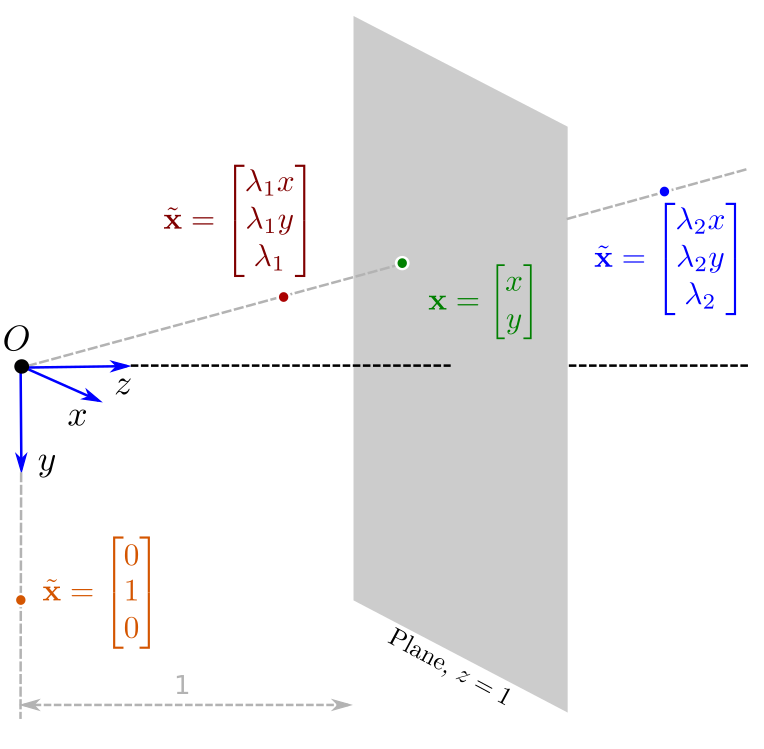
\includegraphics[width=1.0\textwidth]{fig/homogeneous.png}
    \end{columns}
\end{frame}

\begin{frame}
  \frametitle{Camera Model in Homogeneous Coordinates}
  \begin{itemize}[<+->]
    \item Pinhole projection: $\mathbf{x} = \begin{bmatrix}
        \frac{\phi_x u + \gamma v}{w}+\delta_x \\
        \frac{\phi_y v}{w}+\delta_y
      \end{bmatrix}$
    \item In homogeneous coordinates: \begin{equation*}
      \lambda_1 \begin{bmatrix}
        x \\ y \\ 1
      \end{bmatrix} =
      \lambda_2
      \begin{bmatrix}
        \phi_x & \gamma & \delta_x & 0 \\
        0 & \phi_y & \delta_y & 0 \\
        0 & 0 & 1 & 0
      \end{bmatrix} \begin{bmatrix}
        u \\ v \\ w \\ 1
      \end{bmatrix}
      \end{equation*}
    \item Indeed:
      \begin{align*}
        \lambda x &= \phi_x u + \gamma v + \delta_x w \\
        \lambda y &= \phi_y v + \delta_y w \\
        \lambda &= \lambda_1 / \lambda_2 = w
      \end{align*}
  \end{itemize}
\end{frame}

\begin{frame}
  \frametitle{Complete Model}
    \begin{align*}
      \lambda \begin{bmatrix}
        x \\ y \\ 1
      \end{bmatrix} =
      \begin{bmatrix}
        \phi_x & \gamma & \delta_x & 0 \\
        0 & \phi_y & \delta_y & 0 \\
        0 & 0 & 1 & 0
      \end{bmatrix}
      \begin{bmatrix}
        \omega_{11} & \omega_{12} & \omega_{13} & \tau_x \\
        \omega_{21} & \omega_{22} & \omega_{23} & \tau_y \\
        \omega_{31} & \omega_{32} & \omega_{33} & \tau_z \\
        0 & 0 & 0 & 1
      \end{bmatrix} \begin{bmatrix}
        u \\ v \\ w \\ 1
      \end{bmatrix}
      \end{align*}
      \pause
      or
      \begin{align*}
        \mathbf{\tilde{x}} &= \boldsymbol{\Lambda}
        \begin{bmatrix}
          \boldsymbol{\Omega} &
          \bm{\tau}
        \end{bmatrix}
          \mathbf{\tilde{w}}
      \end{align*}
      \pause
      \begin{itemize}
        \item This model will be used to compute good initial estimates
          for the nonlinear optimization problem
      \end{itemize}
\end{frame}

\section{Learning extrinsic parameters}

\begin{frame}
  \frametitle{Learning extrinsic parameters}
  \begin{align*}
    \boldsymbol{\hat{\Omega}},\bm{\hat{\tau}} &=
    \underset{\boldsymbol{\Omega},\bm{\tau}}
    {\operatorname{argmax}} \left[
      \sum_{i=1}^I \log{\left[
    \Pr(\mathbf{x}_i|\mathbf{w}_i,\boldsymbol{\Lambda},\boldsymbol{\Omega},
    \bm{\tau})
      \right]}
    \right]
  \end{align*}
  \pause
  \begin{itemize}
    \item For the $i$th point in homogeneous coordinates:
    \begin{align*}
      \lambda_i \begin{bmatrix}
        x_i \\ y_i \\ 1
      \end{bmatrix} =
      \begin{bmatrix}
        \phi_x & \gamma & \delta_x & 0 \\
        0 & \phi_y & \delta_y & 0 \\
        0 & 0 & 1 & 0
      \end{bmatrix}
      \begin{bmatrix}
        \omega_{11} & \omega_{12} & \omega_{13} & \tau_x \\
        \omega_{21} & \omega_{22} & \omega_{23} & \tau_y \\
        \omega_{31} & \omega_{32} & \omega_{33} & \tau_z \\
        0 & 0 & 0 & 1
      \end{bmatrix} \begin{bmatrix}
        u_i \\ v_i \\ w_i \\ 1
      \end{bmatrix}
      \end{align*}
      \pause
    \item We want to eliminate known $\boldsymbol{\Lambda}$
  \end{itemize}
\end{frame}

\begin{frame}
  \frametitle{Learning extrinsic parameters}
  \begin{itemize}[<+->]
    \item Multiply by $\boldsymbol{\Lambda}^{-1}$:
    \begin{align*}
      \lambda_i \begin{bmatrix}
        x'_i \\ y'_i \\ 1
      \end{bmatrix} =
      \begin{bmatrix}
        \omega_{11} & \omega_{12} & \omega_{13} & \tau_x \\
        \omega_{21} & \omega_{22} & \omega_{23} & \tau_y \\
        \omega_{31} & \omega_{32} & \omega_{33} & \tau_z \\
        0 & 0 & 0 & 1
      \end{bmatrix} \begin{bmatrix}
        u_i \\ v_i \\ w_i \\ 1
      \end{bmatrix}
      \end{align*}
    \item Here $\mathbf{\tilde{x}'} =
      \boldsymbol{\Lambda}^{-1}\mathbf{\tilde{x}}$ are \emph{normalized image
      coordinates}
    \item Now $\lambda_i = \omega_{31}u_i+\omega_{32}v_i+\omega_{33}w_i+\tau_z$

  \end{itemize}
\end{frame}

\setcounter{MaxMatrixCols}{20}

\begin{frame}
  \frametitle{Learning extrinsic parameters}
  \begin{itemize}[<+->]
        \item Substituting back:
          \begin{align*}
          \begin{bmatrix}
            (\omega_{31}u_i+\omega_{32}v_i+\omega_{33}w_i+\tau_z)x'_i \\
            (\omega_{31}u_i+\omega_{32}v_i+\omega_{33}w_i+\tau_z)y'_i
          \end{bmatrix} &=
            \begin{bmatrix}
              \omega_{11} & \omega_{12} & \omega_{13} & \tau_x \\
              \omega_{21} & \omega_{22} & \omega_{23} & \tau_y
            \end{bmatrix}
            \begin{bmatrix}
              u_i \\ v_i \\ w_i \\ 1
            \end{bmatrix}
        \end{align*}
      \item Rearranging for all $i$:
        \tiny{
        \begin{align*}
          \underbrace{
          \begin{bmatrix}
            u_1 & v_1 & w_1 & 1 & 0 & 0 & 0 & 0 &
            -u_1 x_1' & -v_1 x_1' & -w_1 x_1' & -x_1' \\
            0 & 0 & 0 & 0 & u_1 & v_1 & w_1 & 1 &
            -u_1 y_1' & -v_1 y_1' & -w_1 y_1' & -y_1' \\
            u_2 & v_2 & w_2 & 1 & 0 & 0 & 0 & 0 &
            -u_2 x_2' & -v_2 x_2' & -w_2 x_2' & -x_2' \\
            0 & 0 & 0 & 0 & u_2 & v_2 & w_2 & 1 &
            -u_2 y_2' & -v_2 y_2' & -w_2 y_2' & -y_2' \\
                      & & & & & & & \vdots & & & \\
            u_I & v_I & w_I & 1 & 0 & 0 & 0 & 0 &
            -u_I x_I' & -v_I x_I' & -w_I x_I' & -x_I' \\
            0 & 0 & 0 & 0 & u_I & v_I & w_I & 1 &
            -u_I y_I' & -v_I y_I' & -w_I y_I' & -y_I'
          \end{bmatrix}
        }_{
          \mathbf{A}
        }
        \underbrace{
          \begin{bmatrix}
            \omega_{11} \\
            \omega_{12} \\
            \omega_{13} \\
            \tau_x \\
            \omega_{21} \\
            \omega_{22} \\
            \omega_{23} \\
            \tau_y \\
            \omega_{31} \\
            \omega_{32} \\
            \omega_{33} \\
            \tau_z \\
          \end{bmatrix}
        }_{
          \mathbf{b}
        }
          &=
          \mathbf{0}
        \end{align*}
      }
      \end{itemize}
\end{frame}

\newcommand{\norm}[1]{\left\lVert#1\right\rVert}

\begin{frame}
  \frametitle{Computing estimates}
  \begin{itemize}[<+->]
    \item $\mathbf{A} \mathbf{b} = \mathbf{0}$ overdetermined
    \item \emph{Minimum direction problem}:
      $\operatorname{argmin}_\mathbf{b}\norm{\mathbf{Ab}}^2$ subject to
      $\norm{\mathbf{b}} = 1$
    \item Compute singular value decomposition $\mathbf{A} = \mathbf{ULV}^T$
      and set $\mathbf{\tilde{b}}$ to be the last column of $\mathbf{V}$
  \end{itemize}
\end{frame}

\begin{frame}
  \frametitle{Satisfying constraints}
  \begin{itemize}[<+->]
    \item Estimates of $\boldsymbol{\Omega}$ and $\bm{\tau}$ extracted from
      $\mathbf{b}$ have arbitrary scale
    \item $\boldsymbol{\Omega}$ must be a rotation matrix: find "closest" matrix
      to our estimate that satisfies constraints
    \item \emph{Orthogonal Procrustes problem}:
      $\operatorname{argmin}_{\boldsymbol{\Omega}}
      \norm{\boldsymbol{\Omega}-\mathbf{B}}$ subject to
      $\boldsymbol{\Omega\Omega}^T = \mathbf{I}$
    \item Compute SVD $\boldsymbol{\Omega} = \mathbf{ULV}^T$ and set
      $\boldsymbol{\hat{\Omega}} = \mathbf{UV}^T$
    \item Now $\bm{\tau}$ must be scaled:
      $\bm{\hat{\tau}} = \sum_{m=1}^3 \sum_{n=1}^3 \frac{\hat{\Omega}_{mn}}
      {\Omega_{mn}}\bm{\tau}$
    \item Finally, if $\tau_z < 0$ (object behind camera),
      multiply estimates by minus one
  \end{itemize}
\end{frame}

\begin{frame}
  \frametitle{Discussion}
  \begin{itemize}
    \item Very ad hoc algorithm, typical of methods using homogeneous
      coordinates
    \item Can be inaccurate but usually sufficient for an initial guess
    \item Subsequent nonlinear optimization procedure must ensure that
      $\boldsymbol{\Omega}$ remains a valid rotation matrix
    \item The procedure requires at least 6 points for a unique solution (12
      unknowns, 2 equations per point)
  \end{itemize}
\end{frame}

\section{Learning intrinsic parameters}
\section{Inferring 3D world points}
\section{Applications}

\end{document}
